%% LyX 2.3.6.1 created this file.  For more info, see http://www.lyx.org/.
%% Do not edit unless you really know what you are doing.
\documentclass[english]{article}
\usepackage[T1]{fontenc}
\usepackage[latin9]{inputenc}
\usepackage{geometry}
\geometry{verbose,tmargin=2.5cm,bmargin=2.5cm,lmargin=2.5cm,rmargin=2.5cm}
\usepackage{graphicx}
\PassOptionsToPackage{normalem}{ulem}
\usepackage{ulem}

\makeatletter

%%%%%%%%%%%%%%%%%%%%%%%%%%%%%% LyX specific LaTeX commands.
%% Because html converters don't know tabularnewline
\providecommand{\tabularnewline}{\\}

\makeatother

\usepackage{babel}
\begin{document}
{[}SPLIT\_HERE{]}
\begin{enumerate}
\item \textbf{{[}RVHS/PRELIM/9569/2021/P1/Q1{]} }

Draw a reduced decision table based on the following conditions regarding
how John should go to school. \hfill{}{[}5{]}
\begin{itemize}
\item If it is a Monday, John always takes his dad\textquoteright s car
to school if he does not oversleep. 
\item If John oversleeps, he always takes Taxi to school. 
\item Otherwise, if it is a rainy day, John takes Taxi to school. If not,
by MRT. 
\end{itemize}
{[}SPLIT\_HERE{]}
\item \textbf{{[}RVHS/PRELIM/9569/2021/P1/Q2{]} }

The recursive function below helps to check if a password string \texttt{pw}
satisfies certain requirements. The meaning of the function parameters
\texttt{pw}, \texttt{digit}s, \texttt{upper\_l}, \texttt{lower\_l}
and \texttt{length} are password string, minimum number of digits,
minimum number of uppercase letters, minimum number of lowercase letters
and minimum length of the password respectively.

\noindent\begin{minipage}[t]{1\columnwidth}%
\texttt{def check\_pw(pw, digits, upper\_l, lower\_l, length): }

\texttt{\qquad{}if len(pw) == 0: }

\texttt{\qquad{}\qquad{}return digits < 1 and upper\_l < 1 and lower\_l
< 1 and length < 1 }

\texttt{\qquad{}else: }

\texttt{\qquad{}\qquad{}char = pw{[}0{]} }

\texttt{\qquad{}\qquad{}if char.isdigit(): }

\texttt{\qquad{}\qquad{}\qquad{}return check\_pw(pw{[}1:{]}, digits-1,
upper\_l, lower\_l, length-1) }

\texttt{\qquad{}\qquad{}elif char.isalpha(): }

\texttt{\qquad{}\qquad{}\qquad{}if char.isupper():}

\texttt{\qquad{}\qquad{}\qquad{}\qquad{}return check\_pw(pw{[}1:{]},
digits, upper\_l-1, lower\_l, length-1) }

\texttt{\qquad{}\qquad{}\qquad{}else: }

\texttt{\qquad{}\qquad{}\qquad{}\qquad{}return check\_pw(pw{[}1:{]},
digits, upper\_l, lower\_l-1, length-1) }

\texttt{\qquad{}\qquad{}\qquad{}else: }

\texttt{\qquad{}\qquad{}\qquad{}\qquad{}return False }%
\end{minipage}
\begin{enumerate}
\item State the values of all arguments in each recursive function call
when the following code is executed. Then, state the value that the
function returns. 

\texttt{>\textcompwordmark >\textcompwordmark > check\_pw(\textquotedbl SP500\textquotedbl ,
3, 1, 1, 5)} \hfill{}{[}3{]}

The function in \textbf{2a)} is rewritten in such a way that string
slicing on the password string pw is removed. A new function parameter
\texttt{i} is added to help the recursive function to keep track of
the position in \texttt{pw} in which it is currently checking. 

\noindent\begin{minipage}[t]{1\columnwidth}%
\texttt{def check\_pw(pw, i, digits, upper\_l, lower\_l, length): }

\texttt{if}\texttt{\textbf{ }}\texttt{\textbf{\uline{A}}}\texttt{: }

\texttt{\qquad{}return digits < 1 and upper\_l < 1 and lower\_l <
1 and length < 1 }

\texttt{else: }

\texttt{\qquad{}}\texttt{\textbf{\uline{B}}}\texttt{ }

\texttt{\qquad{}if char.isdigit(): }

\texttt{\qquad{}\qquad{}return check\_pw(pw, C, digits-1, upper\_l,
lower\_l, length-1) }

\texttt{\qquad{}elif char.isalpha(): }

\texttt{\qquad{}\qquad{}if char.isupper(): }

\texttt{\qquad{}\qquad{}\qquad{}return check\_pw(pw, C, digits,
upper\_l-1, lower\_l, length-1) }

\texttt{\qquad{}\qquad{}else: }

\texttt{\qquad{}\qquad{}\qquad{}return check\_pw(pw, C, digits,
upper\_l, lower\_l-1, length-1) }

\texttt{\qquad{}\qquad{}else: }

\texttt{\qquad{}\qquad{}\qquad{}return False }%
\end{minipage}
\item State the code in \textbf{A}, \textbf{B} and \textbf{C}. \hfill{}{[}3{]}
\item Describe clearly or write in Python the modification needed for the
function \texttt{check\_pw()} to also display a suggestion of a new
password if the password requirements are not met. For example, if
\texttt{pw} does not have enough digits, it will append digits to
\texttt{pw} so that it can satisfy the requirement. 

For example, 

\texttt{>\textcompwordmark >\textcompwordmark > check\_pw(\textquotedbl WoBeiShiGeDa\textquotedbl ,
0, 2, 6, 7, 15) }

\texttt{Suggested password: WoBeiShiGeDa33Uxxx }

\texttt{False }

\texttt{\textquotedbl 33Uxxx\textquotedbl} is added to \texttt{\textquotedbl WoBeiShiGeDa\textquotedbl}
so that the password passes the requirements. \hfill{}{[}4{]}
\end{enumerate}
{[}SPLIT\_HERE{]}
\item \textbf{{[}RVHS/PRELIM/9569/2021/P1/Q3{]} }

The following recursive procedure is created to encode a character
\texttt{char} based on a \texttt{shift} value. For example, if letter
\textquotedbl\texttt{a}\textquotedbl{} is shifted by \texttt{3},
it will become letter \textquotedbl\texttt{d}\textquotedbl ; and
if shifted by \texttt{-3}, it will become letter \textquotedbl\texttt{x}\textquotedbl . 

The \texttt{ORD} and \texttt{CHR} function will help to convert the
character to its ASCII value and vice versa.

\noindent\begin{minipage}[t]{1\columnwidth}%
\texttt{01 PROCEDURE ENCODE\_CHAR(char: STRING, shift: INT): }

\texttt{02 \qquad{}IF shift == 0: }

\texttt{03 \qquad{}\qquad{}RETURN char }

\texttt{04 \qquad{}ELSE IF shift > 0: }

\texttt{05 \qquad{}\qquad{}DECLARE new\_char: STRING }

\texttt{06 \qquad{}\qquad{}new\_char = CHR((ORD(char) + 1) \% 26) }

\texttt{07 \qquad{}\qquad{}shift -= 1 }

\texttt{08 \qquad{}\qquad{}RETURN ENCODE\_CHAR(new\_char, shift) }

\texttt{09 \qquad{}ELSE: }

\texttt{10 \qquad{}\qquad{}Shift += 26 }

\texttt{11 \qquad{}\qquad{}RETURN ENCODE\_CHAR(char, shift) }

\texttt{12 \qquad{}END IF }

\texttt{13 END PROCEDURE}%
\end{minipage} 
\begin{enumerate}
\item Identify one error from the above code, state the type of the error,
including its definition and explain how the errors can be fixed.
\hfill{}{[}2{]}
\item Assume the above error has been fixed. Copy the following trace table
to your answer booklet. State the line number each time one of the
return statements is called and complete it based on the following
function call. 

\texttt{ENCODE\_CHAR(\textquotedbl y\textquotedbl , -24) }\hfill{}{[}3{]}
\noindent \begin{center}
\begin{tabular}{|c|c|c|c|}
\hline 
\texttt{Line No. } & \texttt{char } & \texttt{shift } & \texttt{new\_char }\tabularnewline
\hline 
 &  &  & \tabularnewline
\hline 
 &  &  & \tabularnewline
\hline 
 &  &  & \tabularnewline
\hline 
\end{tabular}
\par\end{center}

\end{enumerate}
{[}SPLIT\_HERE{]}
\item \textbf{{[}RVHS/PRELIM/9569/2021/P1/Q4{]} }

Answer all questions. 
\begin{center}
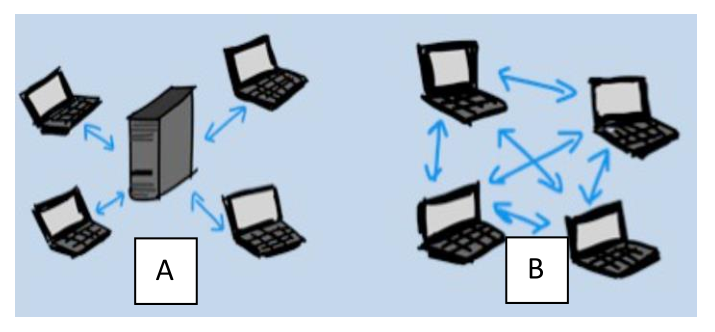
\includegraphics[width=0.5\paperwidth]{C:/Users/Admin/Desktop/Github/question_bank/LyX/static/img/9569-RVHS-2021-P1-Q4}
\par\end{center}
\begin{enumerate}
\item State the network architecture model of A and B as shown in the diagram
below.\hfill{} {[}1{]}
\item State an advantage of model A over B in the diagram above.\hfill{}{[}1{]}
\item State and explain if each of the following statements are correct.
\hfill{}{[}6{]}
\begin{itemize}
\item \textquotedblleft One of the functionalities of the DNS is that different
users can simultaneously receive different IP translations for the
same domain name.\textquotedblright{} 
\item \textquotedblleft The 4 top layers of TCP/IP model are application,
internet, data link and physical.\textquotedblright{} 
\item \textquotedblleft The internet layer is not responsible for reliable
transmission. It makes no guarantees about the proper arrival of packets.\textquotedblright{} 
\item \textquotedblleft 2C:54:91:G8:F9:E3 is a valid MAC address.\textquotedblright{} 
\item \textquotedblleft 2001:0db8:0001:0ab9:C0A8:0102 is a valid IPv6 address.\textquotedblright{} 
\item \textquotedblleft The internet and the World Wide Web are the same
thing.\textquotedblright{} 
\end{itemize}
\item State the purpose of HTTP and explain how the protocol works. \hfill{}{[}3{]}
\item Explain packet switching. \hfill{}{[}1{]}
\item State an ethical issue related to artificial intelligence.\hfill{}
{[}1{]}
\item State the purpose of defining the code of conduct for computer use.
\hfill{}{[}2{]}
\item State a difference between data validation and data verification.\hfill{}
{[}1{]}
\end{enumerate}
{[}SPLIT\_HERE{]}
\item \textbf{{[}RVHS/PRELIM/9569/2021/P1/Q5{]} }

The implementation of a Binary Search Tree (BST) using three 1D arrays
is shown below. 

Each unused node that are not in the logical BST is initially connected
in a singly linked list manner using the \texttt{leftPtr} array. The
first position of this linked list is indicated by the variable \texttt{nextFree}. 

When a piece of data is inserted into the BST, a node will be disconnected
from the linked list and added to the logical BST. The root of this
logical BST is indicated by the variable \texttt{root}. The logical
structure of the BST is managed by \texttt{leftPtr} and \texttt{rightPtr}
which are the positions of the left and right child of the node respectively. 

Below is an illustration for such BST with a 0-based index array. 

\begin{tabular}{|c|c|}
\hline 
\texttt{root } & 7 \tabularnewline
\hline 
\texttt{nextFree} & 0\tabularnewline
\hline 
\end{tabular} 

\begin{tabular}{|c|c|c|c|c|c|c|c|c|}
\hline 
Array Index  & 0 & 1 & 2 & 3 & 4 & 5 & 6 & 7\tabularnewline
\hline 
\texttt{Data } & - & 7 & 10 & 6 & 1 & 4 & 2 & 9\tabularnewline
\hline 
\texttt{leftPtr } & -1 & -1 & -1 & 5 & -1 & 6 & 4 & 3\tabularnewline
\hline 
\texttt{rightPtr } & -1 & -1 & -1 & 1 & -1 & -1 & -1 & 2\tabularnewline
\hline 
\end{tabular}
\begin{enumerate}
\item Draw the logical BST at this point of time. \hfill{}{[}1{]}
\item State the post order traversal of the BST \hfill{}{[}1{]}
\item State the values of \texttt{root}, \texttt{nextFree} and the values
in the arrays \texttt{data}, \texttt{leftPtr} and \texttt{rightPtr}
after the \textbf{each} of the following BST operations are executed
sequentially. \hfill{}{[}3{]} 
\begin{itemize}
\item \texttt{Add 8}
\item \texttt{Recursive Delete 6 }
\end{itemize}
\item State an advantage of BST over Hash table. \hfill{}{[}1{]}
\item Explain what can make a Hash Table Search inefficient besides a bad
hash function and how to overcome it. \hfill{}{[}2{]}
\item State 2 characteristics of a good hash function. \hfill{}{[}2{]}
\end{enumerate}
{[}SPLIT\_HERE{]}
\item \textbf{{[}RVHS/PRELIM/9569/2021/P1/Q6{]} }

Study the following sorting code carefully. 

\noindent %
\noindent\begin{minipage}[t]{1\columnwidth}%
\texttt{def sort(lst): }

\texttt{\qquad{}if len(lst)<=1: }

\texttt{\qquad{}\qquad{}return lst }

\texttt{\qquad{}else: }

\texttt{\qquad{}\qquad{}pivot = lst{[}0{]} }

\texttt{\qquad{}\qquad{}smaller = {[}{]} }

\texttt{\qquad{}\qquad{}larger = {[}{]} }

\texttt{\qquad{}\qquad{}for i in range (1, len(lst)): }

\texttt{\qquad{}\qquad{}\qquad{}if lst{[}i{]} < pivot: }

\texttt{\qquad{}\qquad{}\qquad{}\qquad{}smaller.append(lst{[}i{]}) }

\texttt{\qquad{}\qquad{}\qquad{}else: }

\texttt{\qquad{}\qquad{}\qquad{}\qquad{}larger.append(lst{[}i{]}) }

\texttt{\qquad{}\qquad{}return sort (smaller) + {[}pivot,{]} + sort
(larger) }%
\end{minipage}
\begin{enumerate}
\item State the name of the above sorting algorithm. \hfill{}{[}1{]}
\item Explain why the above sorting algorithm is inefficient when it is
used on a nearly sorted array. \hfill{} {[}1{]}
\item Explain how you can modify the code to improve the efficiency. \hfill{}{[}2{]}
\end{enumerate}
Bubble sort and insertion sort are both used to sort a nearly sorted
integer array of size 1000 and there are only 5 integers in the array
that are not in the correct position. 
\begin{enumerate}
\item State and explain why insertion sort generally perform better than
bubble sort for nearly sorted array. \hfill{}{[}2{]}
\item Draw a flow chart for the algorithm described below. \hfill{}{[}4{]}

Given an integer \texttt{k} and an array \texttt{arr{[}{]}} representing
the destination floors for \texttt{n} people waiting currently at
the ground floor and \texttt{k} is the capacity of the elevator. It
takes 1 unit time for the elevator to reach any consecutive floor
from the current floor. The algorithm finds the minimal time taken
to get all the people to their destination floor and then return to
the ground floor. 

\noindent\begin{minipage}[t]{1\columnwidth}%
\texttt{def minTime(n, k, arr) : }

\texttt{\qquad{}\# Sort in descending order }

\texttt{\qquad{}arr.sort(reverse = True) }

\texttt{\qquad{}minTime = 0 }

\texttt{\qquad{}\# Iterate through the groups }

\texttt{\qquad{}for i in range(0, n, k) : }

\texttt{\qquad{}\qquad{}\# Update the time taken for }

\texttt{\qquad{}\qquad{}\# each group }

\texttt{\qquad{}\qquad{}minTime += (2 {*} arr{[}i{]}) }

\texttt{\qquad{}\# Return the total time taken }

\texttt{\qquad{}return minTime}%
\end{minipage} 
\end{enumerate}
{[}SPLIT\_HERE{]}
\item \textbf{{[}RVHS/PRELIM/9569/2021/P1/Q7{]} }

A relational database is created to store data about contractors engaging
workers to perform renovation jobs. 

The database designers are told that: 
\begin{itemize}
\item each contractor can recruit different workers to perform various jobs.
\item each worker can have skills to perform different jobs. 
\item each job can have different levels of skills \textquotedbl A\textquotedbl ,
\textquotedbl B\textquotedbl{} or \textquotedbl C\textquotedbl{}
and their hourly rate is calculated based on their skill level for
the job. 
\end{itemize}
A first attempt is represented by the following table: 
\begin{center}
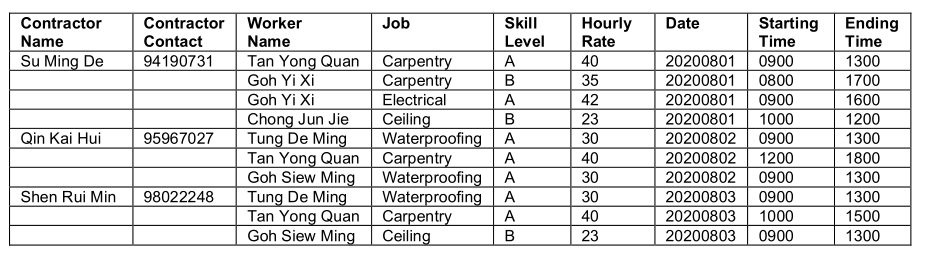
\includegraphics[width=0.65\paperwidth]{C:/Users/Admin/Desktop/Github/question_bank/LyX/static/img/9569-RVHS-2021-P1-Q7-1}
\par\end{center}
\begin{enumerate}
\item Explain why this table is not in first normalized form. \hfill{}{[}2{]}
\end{enumerate}
The following is an attempt to reduce data redundancy: 
\begin{center}
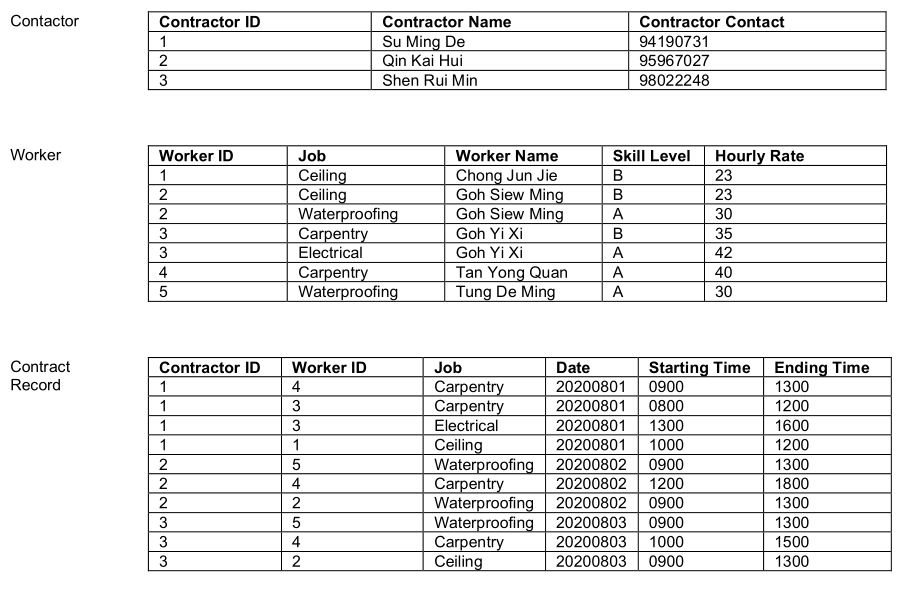
\includegraphics[width=0.65\paperwidth]{C:/Users/Admin/Desktop/Github/question_bank/LyX/static/img/9569-RVHS-2021-P1-Q7-2}
\par\end{center}
\begin{enumerate}
\item[(b)] Explain what a composite key is. \hfill{}{[}1{]}
\item[(c)] State a suitable primary key for Worker table and explain why the
table is not in second normal form. \hfill{}{[}3{]}
\item[(d)] A table description can be expressed as: 

\texttt{TableName (}\texttt{\uline{Attribute1}}\texttt{, Attribute2{*},
Attribute3, \dots ) }

The primary keys are indicated using a solid underline and foreign
keys are indicated by using a dashed underline/asterisk. Write table
descriptions for the required tables in the database so that they
are in third normal form (3NF). \hfill{} {[}6{]}
\item[(d)] Create an entity-relationship (ER) diagram showing the degree of
all relations. \hfill{}{[}3{]}
\item[(e)] Using the above example, elaborate why a relational database model
has advantage in maintaining data integrity over a flat file system.
\hfill{}{[}3{]}
\item[(f)] The homeowner would like to know a schedule of the renovation jobs
performed to their house. They are \textbf{NOT} interested in knowing
the exact worker\textquoteright s name. Write an SQL query to output
the \textbf{contractor\textquoteright s name}, \textbf{worker\textquoteright s
job}, \textbf{worker\textquoteright s skill level} and \textbf{date}
based on the contractor\textquoteright s name \textquotedbl\texttt{Su
Ming De}\textquotedbl . The output is to be in the ascending order
based on the date of job performed. \hfill{}{[}5{]}
\end{enumerate}
{[}SPLIT\_HERE{]}
\item \textbf{{[}RVHS/PRELIM/9569/2021/P1/Q8{]} }

You are also to design an Object-Oriented solution for the above-mentioned
project. Both contractor and workers are to create a \texttt{User}
account on the platform, with details such as \texttt{user\_id}, \texttt{password}
and \texttt{gender}. 

The contractors will have to register their company details such as
company \texttt{name} and \texttt{address}, while the workers need
to register their bank \texttt{account} number. 
\begin{enumerate}
\item Draw a class diagram, with base class \textbf{User}, showing: 
\begin{itemize}
\item appropriate sub-classes, 
\item inheritance, 
\item the properties required, 
\item appropriate methods, including but not limited to the \textbf{constructor}
methods, and at least \textbf{one} pair of \textquoteleft \textbf{get}\textquoteright{}
and \textquoteleft \textbf{set}\textquoteright{} methods for each
class, 
\item circle the polymorphed methods. \hfill{} {[}6{]}
\end{itemize}
\item Using the above example, state the definition of inheritance and explain
its purpose/advantage in object-oriented programing. \hfill{} {[}3{]}
\end{enumerate}
The platform hopes to expand its function to allow register of homeowner
accounts. The homeowners can view which are the workers came to their
home address for renovation work on the date/time specified by the
contractors. 
\begin{enumerate}
\item[(c)] State how this would affect the class, properties and methods in
the current example. \hfill{} {[}3{]}
\item[(d)] State how this would affect the tables, attributes and relationships
of the relational database stated in \textbf{7(d)} and \textbf{(e)}.
\hfill{} {[}3{]}
\item[(e)] Explain how NoSQL addresses shortcomings of relational databases.
\hfill{} {[}4{]}
\end{enumerate}
Some homeowners request to have access to the hourly rate and personal
contact of renovation workers. 
\begin{enumerate}
\item[(f)]  From the perspective of the company, explain to the homeowners how
such a feature is against the data protection obligations stated in
the Personal Data Protection Act (PDPA). \hfill{} {[}2{]}
\end{enumerate}
{[}SPLIT\_HERE{]}
\item \textbf{{[}RVHS/PRELIM/9569/2021/P2/Q1{]} }

\textbf{Task 1.1}

Write a function \texttt{task1\_1(name\_A, name\_B)} where \texttt{name\_A}
and \texttt{name\_B} are strings which consists of only alphabet letters
and spaces. The function will return \texttt{True} if 
\begin{itemize}
\item the alphabet letters combination used in string \texttt{name\_A} and
\texttt{name\_B} are the same and
\item the spaces in string \texttt{name\_A} and \texttt{name\_B} are at
the same locations. \hfill{}{[}7{]}
\end{itemize}
For example, 

\noindent %
\noindent\begin{minipage}[t]{1\columnwidth}%
\texttt{>\textcompwordmark >\textcompwordmark > match\_names(\textquotedbl Abcde\textquotedbl ,
\textquotedbl Deabc\textquotedbl ) }

\texttt{True }

\texttt{>\textcompwordmark >\textcompwordmark > match\_names(\textquotedbl Abcde
Fgh I\textquotedbl , \textquotedbl Ihgfe Dcb A\textquotedbl ) }

\texttt{True }

\texttt{>\textcompwordmark >\textcompwordmark > match\_names(\textquotedbl Abcd
Efgh I\textquotedbl , \textquotedbl Ihgfe Dcb A\textquotedbl ) }

\texttt{False }

\texttt{>\textcompwordmark >\textcompwordmark > match\_names(\textquotedbl Abcde
Fzh I\textquotedbl , \textquotedbl Ihgfe Dcb A\textquotedbl ) }

\texttt{False} %
\end{minipage}

Test your program with the following test data: 

\noindent\begin{minipage}[t]{1\columnwidth}%
\texttt{print(task1\_1(\textquotedbl Abcde\textquotedbl , \textquotedbl Deabc\textquotedbl )) }

\texttt{print(task1\_1(\textquotedbl Abcde Fgh I\textquotedbl ,
\textquotedbl Ihgfe Dcb A\textquotedbl )) }

\texttt{print(task1\_1(\textquotedbl Abcd Efgh I\textquotedbl ,
\textquotedbl Ihgfe Dcb A\textquotedbl )) }

\texttt{print(task1\_1(\textquotedbl Abcde Fzh I\textquotedbl ,
\textquotedbl Ihgfe Dcb A\textquotedbl ))}%
\end{minipage} 

\subsubsection*{Task 1.2 }

Write the function \texttt{task1\_2()} to read the names in file \texttt{\textquotedbl namelist\_A.txt\textquotedbl}
and find a matching name in \textquotedbl\texttt{namelist\_B.txt}\textquotedbl{}
that satisfied the conditions stated in \textbf{Task 1.1}. If a matching
name cannot be found in \textquotedbl\texttt{namelist\_B.txt}\textquotedbl ,
it will just display \textquotedbl\texttt{{*}{*}{*}{*}{*}{*}{*}{*}{*}{*}{*}No
match{*}{*}{*}{*}{*}{*}{*}{*}{*}{*}{*}}\textquotedbl . Your results
should be displayed in the following manners. The time-complexity
of your program code matters. \hfill{}{[}13{]}
\begin{center}
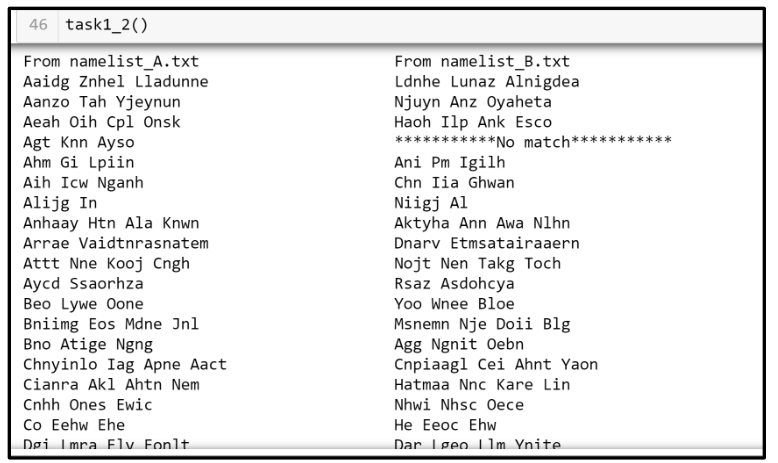
\includegraphics[width=0.5\paperwidth]{C:/Users/Admin/Desktop/Github/question_bank/LyX/static/img/9569-RVHS-2021-P2-Q1}
\par\end{center}

{[}SPLIT\_HERE{]}
\item \textbf{{[}RVHS/PRELIM/9569/2021/P2/Q2{]} }

\textbf{Task 2.1}

Complete the doubly linked list class \texttt{Doubly\_LL} by implementing
both the \texttt{insert} and \texttt{delete} class functions. \hfill{}{[}10{]}
\begin{itemize}
\item The class function \texttt{insert(node)} takes a \texttt{Node} instance
\texttt{node} as input and inserts it at the tail of the linked list.
Take note that the attributes \texttt{prev} and \texttt{next} of \texttt{Node}
instance \texttt{node} are both \texttt{None} before the insertion. 
\item The class function \texttt{delete(node)} takes a \texttt{Node} instance
\texttt{node} which exists in the linked list as input. The function
removes/detaches \texttt{node} from the linked list and returns it.
The \texttt{node} returned has both its attributes \texttt{prev} and
\texttt{next} set to \texttt{None}, but data remains unchanged. 
\end{itemize}

\subsubsection*{Task 2.2 }

The class \texttt{LRUQ} uses the doubly linked list class \texttt{Doubly\_LL}
to implement its least recently used queue (\texttt{lruq}). \hfill{}{[}8{]}
\begin{itemize}
\item The attribute hashmap is a dictionary object that takes the node's
data as key and the node instance itself in lruq as value. 
\item The attribute size is the max number of nodes that lruq can have.
\item The attribute count is the number of nodes that lruq currently have. 
\end{itemize}
Complete the least recently used queue class \texttt{LRUQ} by implementing
the \texttt{use} function. The class function \texttt{use(value)}
takes an integer \texttt{value} as input. 
\begin{itemize}
\item If \texttt{value} is in \texttt{lruq} (referenced by hashmap), it
removes the node in the \texttt{lruq} and re-insert it to the end
of the \texttt{lruq}. 
\item If \texttt{value} is not in \texttt{lruq} (not referenced by hashmap),
it references \texttt{value} in hashmap and inserts a new \texttt{Node}
instance with value as its data to the end of \texttt{lruq}. If \texttt{count}
> \texttt{size}, it removes the least recently used node in \texttt{lruq}
and de-references it in \texttt{hashmap}. 

Hint: To de-reference a key in \texttt{hashmap}, you can call the
following. \texttt{self.hashmap.pop(key, None)} where \texttt{self.hashmap}
is a dictionary object. 
\end{itemize}
The test function \texttt{test2\_2()} is provided for you in \texttt{task2.ipynb}.
The expected outcome of this test function is shown on the next page.
Take note that the size of the least recently used queue is \texttt{6}
in this test function. 

\noindent %
\noindent\begin{minipage}[t]{1\columnwidth}%
\texttt{Latest item used: 3 }

\texttt{From least recently used to most recently used: Print from
head: }

\texttt{3 }

\texttt{-{}-{}-{}-{}-{}-{}-{}-{}-{}-{}-{}-{}-{}-{}-{}- }

\texttt{Latest item used: 8 }

\texttt{From least recently used to most recently used: Print from
head: 3 8 }

\texttt{-{}-{}-{}-{}-{}-{}-{}-{}-{}-{}-{}-{}-{}-{}-{}- }

\texttt{Latest item used: 2 }

\texttt{From least recently used to most recently used: Print from
head: }

\texttt{3 8 2 }

\texttt{-{}-{}-{}-{}-{}-{}-{}-{}-{}-{}-{}-{}-{}-{}-{}- }

\texttt{Latest item used: 45 }

\texttt{From least recently used to most recently used: Print from
head: }

\texttt{3 8 2 45 }

\texttt{-{}-{}-{}-{}-{}-{}-{}-{}-{}-{}-{}-{}-{}-{}-{}- }

\texttt{Latest item used: 3 }

\texttt{From least recently used to most recently used: Print from
head: }

\texttt{8 2 45 3}

\texttt{-{}-{}-{}-{}-{}-{}-{}-{}-{}-{}-{}-{}-{}-{}-{}- }

\texttt{Latest item used: 45 }

\texttt{From least recently used to most recently used: Print from
head: }

\texttt{8 2 3 45 }

\texttt{-{}-{}-{}-{}-{}-{}-{}-{}-{}-{}-{}-{}-{}-{}-{}- }

\texttt{Latest item used: 45 }

\texttt{From least recently used to most recently used: Print from
head: }

\texttt{8 2 3 45 }

\texttt{-{}-{}-{}-{}-{}-{}-{}-{}-{}-{}-{}-{}-{}-{}-{}- }

\texttt{Latest item used: 12 }

\texttt{From least recently used to most recently used: }

\texttt{Print from head: 8 2 3 45 12 }

\texttt{-{}-{}-{}-{}-{}-{}-{}-{}-{}-{}-{}-{}-{}-{}-{}- }

\texttt{Latest item used: 31 }

\texttt{From least recently used to most recently used: Print from
head: }

\texttt{8 2 3 45 12 31 }\textbf{//Queue is full at this point}

\texttt{-{}-{}-{}-{}-{}-{}-{}-{}-{}-{}-{}-{}-{}-{}-{}- }

\texttt{Latest item used: 42 }

\texttt{From least recently used to most recently used: Print from
head: }

\texttt{2 3 45 12 31 42 }\textbf{//8 is removed because it is the
least used }

\texttt{-{}-{}-{}-{}-{}-{}-{}-{}-{}-{}-{}-{}-{}-{}-{}- }

\texttt{Latest item used: 12 }

\texttt{From least recently used to most recently used: Print from
head: }

\texttt{2 3 45 31 42 12 }

\texttt{-{}-{}-{}-{}-{}-{}-{}-{}-{}-{}-{}-{}-{}-{}-{}- }

\texttt{Latest item used: 12 }

\texttt{From least recently used to most recently used: Print from
head:}

\texttt{2 3 45 31 42 12 }

\texttt{-{}-{}-{}-{}-{}-{}-{}-{}-{}-{}-{}-{}-{}-{}-{}- }

\texttt{Latest item used: 2 }

\texttt{From least recently used to most recently used: Print from
head: }

\texttt{3 45 31 42 12 2 }

\texttt{-{}-{}-{}-{}-{}-{}-{}-{}-{}-{}-{}-{}-{}-{}-{}- }%
\end{minipage}

{[}SPLIT\_HERE{]}

\item \textbf{{[}RVHS/PRELIM/9569/2021/P2/Q3{]} }

\textbf{Task 3.1}

Write program code to read the csv file \textquotedbl\texttt{health\_facilities.csv}\textquotedbl{}
and insert all information in the file as documents into a NoSQL MongoDB
database called \textquotedbl\texttt{Health}\textquotedbl{} with
one collection called \textquotedbl\texttt{facilities}\textquotedbl .
The \textquotedbl\texttt{\_id}\textquotedbl{} of the documents in
the database should start from \texttt{1}, \texttt{2}, \texttt{3}
and \texttt{4} etc. The correct data type of each field is expected
to be inserted into the database. \hfill{}{[}10{]}

\subsubsection*{Task 3.2 }
\begin{enumerate}
\item Write a MongoDB Pymongo query to retrieve all public acute hospital
documents with their corresponding number of beds more than 7200.
\hfill{}{[}4{]}
\item Write program code to bubble sort the results retrieved in \textbf{Task
3.2 a)} according to the average number of beds per facility. Then,
display the top 3 years which has the highest average number of beds
per facility using the format below. 

\texttt{The three years that have the highest average number of beds
per facility are: \_\_\_\_\_, \_\_\_\_\_ and \_\_\_\_\_. }

\hfill{}{[}7{]}
\end{enumerate}

\subsubsection*{Task 3.3}
\begin{enumerate}
\item Write a MongoDB Pymongo query and program code to display all \textquotedbl\texttt{\_id}\textquotedbl s
of Not-for-Profit health facilities documents that have no facility.
\hfill{}{[}3{]} 
\item Write MongoDB Pymongo code to update the fields \textquotedbl\texttt{no\_of\_facilities}\textquotedbl{}
and \textquotedbl\texttt{no\_beds}\textquotedbl{} of only 3 documents
retrieved in \textbf{Task 3.3 a)} to \texttt{1} and a random number
from \texttt{10} to \texttt{20} respectively. \hfill{}{[}6{]} 
\end{enumerate}
{[}SPLIT\_HERE{]}
\item \textbf{{[}RVHS/PRELIM/9569/2021/P2/Q4{]} }

\textbf{Car Loaning System }

CaRent is a company providing electronic car rental services. The
company engages you to design a web application using Flask microframework
to aid in the car rental process. 

The following information of each Customer is stored: 

\texttt{CustomerID} -- auto increment integer value to keep track
of the ID of customer. 

\texttt{Name} -- name of customer. 

\texttt{Gender} -- gender of customer, to be stored as a single character,
using either '\texttt{M}' or '\texttt{F}'. 

\texttt{Contact} -- contact number of customer. 

The following information of each Car is stored: 

\texttt{VIN} -- vehicle identification number (VIN) of the car. 

\texttt{Brand} -- brand of the car. 

\texttt{Vehicle Type} -- type of the car, can be \texttt{'Sedan'},
\texttt{'Hatchback'}, \texttt{'SUV'} or \texttt{'MPV'}. 

\texttt{Energy Source} -- type of energy source the engine is running
on, can be \texttt{'Diesel'}, \texttt{'Gasoline'}, \texttt{'Hybrid'}
or \texttt{'Electricity'}. 

\texttt{DailyPrice} -- daily price for renting the car. 

\texttt{Availability} -- availability of the car, can be \texttt{'Available'}
or \texttt{'Unavailable'}. 

The following information of each RentalPoint is stored: 

\texttt{PointID} -- auto increment integer value to keep track of
the ID of rental service point.

\texttt{Address} -- address of the rental point. 

\texttt{OpWeekDay} -- weekdays that the rental point is open, stored
as a 7-digits string, starting from Sunday to Saturday, with \texttt{'1'}
indicating open and \texttt{'0'} indicating closed. E.g. \texttt{'0111110'}
means it is open on weekdays and closed on weekend. 

\texttt{OpStartHr} -- starting time of daily operation, stored as
a 4 digits string, using 24hour time format. 

\texttt{OpEndHr} -- ending time of daily operation, stored as a 4
digits string, using 24hour time format. 

The following information of each \texttt{RentalRecord} is stored: 

\texttt{CustomerID} -- ID of customer. 

\texttt{VIN} -- VIN of car. 

\texttt{StartDate} -- start date for the rental service. 

\texttt{CollectionPointID} -- ID of the collection point. 

\texttt{ReturnDate} -- return date for the rental service. 

\texttt{ReturnPointID} -- ID of the return point. 

The information is to be stored in four tables: 

\texttt{Customer} 

\texttt{Car} 

\texttt{RentalPoint} 

\texttt{RentalRecord} 

\subsubsection*{Task 4.1 }

Create an SQL file called \texttt{Task4\_1.sql} to show the SQL code
to create the database \texttt{car\_rental.db} with the three tables. 

The table \texttt{Customer} must use \texttt{CustomerID} as its primary
key, the table \texttt{Car} must use \texttt{VIN} as its primary key,
and the table \texttt{RentalPoint} must use \texttt{PointID} as its
primary key. 

The table \texttt{RentalRecord} should use \texttt{CustomerID}, \texttt{VIN}
and \texttt{StartDate} as a composite key, while \texttt{CustomerID},
\texttt{VIN} and \texttt{CollectionPointID/ReturnPointID} must refer
to \texttt{CustomerID} in \texttt{Customer}, \texttt{VIN} in \texttt{Car}
and \texttt{PointID} in \texttt{RentalPoint} as foreign keys. 

Save your SQL code as \texttt{Task4\_1.sql} \hfill{} {[}6{]}

\subsubsection*{Task 4.2 }

The files \texttt{customers.csv}, \texttt{cars.csv}, \texttt{rental\_points.csv}
and \texttt{rental\_records.csv} contains information about the customers,
cars, rental points and the past rental records. The first row of
each file contains the header of the respective columns. Each row
in the files is a comma- separated list of information. 

Write a Python program to insert all information from the three files
into the \texttt{database car\_rental.db}. Run the program. 

Save your program code as \texttt{Task4\_2.py} \hfill{}{[}6{]}

\subsubsection*{Task 4.3 }

You are tasked to implement a function to search and display all past
rental records of a customer. Using the customer\textquoteright s
name \texttt{\textbf{'Goh Yi Xi'}}, query and display a list of data
with the following fields as shown in the table, sorted in the ascending
order according to the start date. 
\noindent \begin{center}
\begin{tabular}{|c|c|c|c|c|c|}
\hline 
Name  & Contact  & VehicleType  & StartDate  & ReturnDate  & DailyPrice\tabularnewline
\hline 
\dots{}  & \dots{} & \dots{}  & \dots{}  & \dots{} & \dots{}\tabularnewline
\hline 
\end{tabular}
\par\end{center}

Write the SQL code required. 

Save this code as \texttt{Task4\_3.sql} \hfill{} {[}5{]}

\subsubsection*{Task 4.4 }

The company wants to implement a function to register new cars for
rental into the database. Office staff can register new cars by adding
the values of the attributes in the \texttt{Car} table. 

Write a Python program and the necessary files to create a web application
that: 
\begin{itemize}
\item Receive the following information: 
\begin{itemize}
\item \texttt{VIN}, \texttt{Brand}, \texttt{VehicleType}, \texttt{EnergySource},
and \texttt{DailyPrice} of a car through a HTML form.
\item \texttt{Availability} should be set to the default value of \texttt{'Available'}. 
\item Note that \texttt{VehicleType} and \texttt{EnergySource} should be
in \textbf{dropdown} list format to improve data validity. 
\end{itemize}
\item Check if the \texttt{VIN} is valid based on the following algorithm: 
\begin{itemize}
\item Step 1: Translate all letters to integer values using the following
table (\texttt{I}, \texttt{O}, and \texttt{Q} are not allowed in a
valid \texttt{VIN}): 
\noindent \begin{center}
\begin{tabular}{|c|c|c|c|c|c|c|c|c|}
\hline 
\textbf{A}: 1  & \textbf{B}: 2  & \textbf{C}: 3  & \textbf{D}: 4  & \textbf{E}: 5  & \textbf{F}: 6  & \textbf{G}: 7  & \textbf{H}: 8  & \textbf{N/A}\tabularnewline
\hline 
\textbf{J}: 1  & \textbf{K}: 2  & \textbf{L}: 3  & \textbf{M}: 4  & \textbf{N}: 5  & \textbf{N/A}  & \textbf{P}: 7  & \textbf{N/A } & \textbf{R}: 9\tabularnewline
\hline 
\textbf{N/A}  & \textbf{S}: 2  & \textbf{T}: 3  & \textbf{U}: 4  & \textbf{V}: 5  & \textbf{W}: 6  & \textbf{X}: 7  & \textbf{Y}: 8 & \textbf{Z}: 9\tabularnewline
\hline 
\end{tabular}
\par\end{center}
\item Step 2: Use the following weight factor for each position in the VIN.
\textbf{The 9th position is that of the check digit}. Its weight factor
has been substituted with a \texttt{0}, which will cancel it out in
the multiplication step. 
\noindent \begin{center}
\begin{tabular}{|c|c|c|c|c|c|c|c|c|c|c|c|c|c|c|c|c|c|}
\hline 
\textbf{Position } & \textbf{1 } & \textbf{2 } & \textbf{3} & \textbf{4} & \textbf{5} & \textbf{6} & \textbf{7} & \textbf{8} & \textbf{9} & \textbf{10} & \textbf{11} & \textbf{12} & \textbf{13} & \textbf{14} & \textbf{15} & \textbf{16} & \textbf{17}\tabularnewline
\hline 
Weight  & 8  & 7  & 6  & 5  & 4  & 3  & 2  & 10  & 0  & 9  & 8  & 7  & 6  & 5 & 4 & 3 & 2\tabularnewline
\hline 
\end{tabular}
\par\end{center}
\item The sum of product of the letter/digit with their corresponding weight
factor is then divided by \texttt{11}. 
\item The remainder is the check digit. If the remainder is \texttt{10},
the check digit will use \texttt{X} instead. 
\item E.g. the \texttt{VIN} with values 1\texttt{M8GDM9A\_KP042788} will
produce a check digit of \texttt{X} and hence \texttt{1M8GDM9AXKP042788}
is a valid \texttt{VIN}. 
\end{itemize}
\item If \texttt{VIN} is valid, create a new car record in the \texttt{Car}
table, and display the record in the confirmation page. 
\item Otherwise, inform the user that the VIN is invalid. 
\end{itemize}
\begin{center}
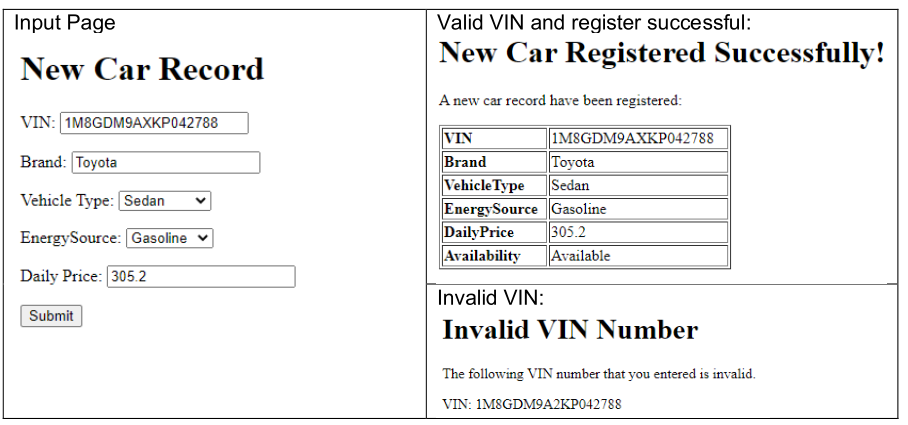
\includegraphics[width=0.5\paperwidth]{C:/Users/Admin/Desktop/Github/question_bank/LyX/static/img/9569-RVHS-2021-P2-Q4}
\par\end{center}

You may assume: 
\begin{itemize}
\item All inputs are in valid format. 
\item VIN: 1M8GDM9AXKP042788 is a new record to the database 
\end{itemize}
Save your program as \texttt{Task4\_4.py }

With additional files or sub-folders as needed in a folder named \texttt{Task4\_4 }

Run the web application. Enter the values based on the sample input
above. 

Then save the output of the program as \texttt{Task4\_4.html}. \hfill{}{[}15{]}

{[}SPLIT\_HERE{]}
\end{enumerate}
 
\end{document}
